
\section{Optimal Reconfiguration of Optimal Ladder Lotteries}
A local swap operation, corresponding to a braid relation in algebra, is a local modification of a ladder lottery 
demonstrated in Figure~\ref{Fig:LocalSwap}~\cite{A1}.
\begin{figure}[h]
    \centering 
    \resizebox{!}{.3\textheight}{
            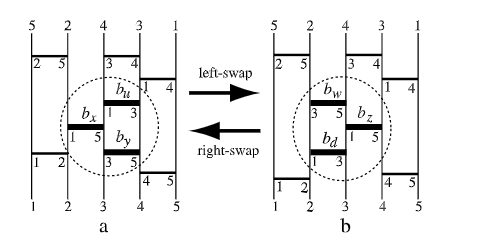
\includegraphics{LocalSwapOperation}
    }
    \caption{A local swap operation}
    \label{Fig:LocalSwap}
\end{figure}

In \emph{Optimal Reconfiguration of Optimal Ladder Lotteries}~\cite{A2}, written by Horiyama, Wasa and Yamanaka,
the authors provide a polynomial solution to the 
Minimal Reconfiguration Problem which asks, given 
two ladders, $L_{i}$ and  $L_{m}$, what is the minimal number of 
swap operations to perform that will transition from $L_{i}$ to $L_{m}$? A \emph{reverse triple} 
is a relation between three bars, $x,y,z$ in two arbitrary ladders, $L_{i}, L_{m}$, such that if $x,y,x$
are right swapped in $L_{i}$, then they are left swapped in $L_{m}$ or if they are 
left swapped in $L_{i}$ then they are right swapped in $L_{m}$. 
Let an \emph{improving triple} be defined as  
performing a right/left swapping three bars, $x,y,z$, in $L_{i}$ such that the 
result of the swap removes a reverse triple between
ladders $L_{i}$ and $L_{m}$. The improving triple is a symmetric 
relation, therefore performing a right/left swapping of the $x,y,z$ in $L_{m}$ also results in the 
removal of a reverse triple between $L_{i}$ and $L_{m}$.\par
The \emph{minimal length reconfiguration sequence} is the minimal number of 
improving triples required to transition from $L_{i}$ to $L_{m}$ or 
$L_{m}$ to $L_{i}$. Transitioning from $L_{i}$ to $L_{m}$ with the minimal length reconfiguration sequence 
is achieved by applying an improving triple to each of the reverse triples between 
$L_{i}$ and $L_{m}$. That is to say, the length of the reconfiguration sequence 
is equal to the number of improving triples required to remove all reverse triples between $L_{i}$ and  $L_{m}$.\par
The second contribution of this paper is that it provides a closed form formula for the 
upper bound for the minimal length reconfiguration sequence for any permutation 
of size $n$. That is to say, given some arbitrary $\pi$ of order $n$, what is the maximum 
number of swaps required for the minimal length reconfiguration sequence between any two ladders in $OptL\{\pi\}$?
The authors prove that there are two unique ladders in $OptL\{(n, n-1, \dots, 1)\}$ that 
have the upper bound for the minimal length reconfiguration sequence. These ladders are the root ladder and \emph{final ladder} 
which is defined as the unique ladder in $OptL\{\pi\}$ such that $\forall z < y < x: (y,z) \text{ is above } (x,z) \in l$. 
The length of the reconfiguration sequence 
between the root ladder and final ladder in $OptL\{(n, n-1, \dots, 1)\}$ is $n{n-1~\choose 2}$. 
